\subsection{Extensibility}
\label{design:extensibility}

The requirements for the bootware component state that support for different cloud environments and provisioning engines should be achieved through means of software engineering.
This requirement is intentionally vague to allow to select a fitting extension mechanism during the design process.

\subsubsection{Extension Mechanisms}

\textcolor{red}{other mechanisms?}

One possibility that would satisfy this criteria is to design interfaces for all extension points of the bootware component.
New cloud environments, provisioning engines, or other extension could then implement these interfaces.
The disadvantage of this approach is that the whole bootware component has to be recompiled, redistributed and redeployed if one extension is added or changed.

To remove this disadvantage, a more flexible architecture is needed, for example a plugin architecture. (\textcolor{red}{pattern?})
Interfaces for the extension points still exist but the extension are no longer part of the main bootware component.
They are compiled separately into plugins that can be loaded into the main bootware component on the fly.
There are several possibilities to realize such an architecture.

It is certainly possible to implement a plugin framework from scratch.
An advantage of this approach would be that the design of the plugin architecture could be tailored to our use case and would be as simple or complex as needed.
But there are also several disadvantages.
For one, we would reinvent the wheel, since multiple such frameworks already exist.
It would also shift resources away from the actual goal of this thesis, which is designing the bootware component.
Furthermore it would require a deep understanding of the language used for the implementation (\textcolor{red}{in this case Java}), which is not necessarily given.
Therefore it seems more reasonable to use one of the already existing plugin frameworks.Three such alternatives will be compared next. (\textcolor{red}{more?})

\subsubsection{Plugin Frameworks}

\begingroup
	\centering
	\captionsetup{type=table}
	\begin{tabu}[!htbp]{rl|[0.5pt]ccc}

		&
		& \multicolumn{3}{c}{\textit{Plugin Frameworks}} \\

		&
		& \begin{sideways} \textbf{JSPF\footnote{\url{https://code.google.com/p/jspf/}\label{jspf}}} \end{sideways}
		& \begin{sideways} \textbf{JPF\footnote{\url{http://jpf.sourceforge.net/}\label{jpf}}} \end{sideways}
		& \begin{sideways} \textbf{OSGi\footnote{\url{http://www.osgi.org/}\label{osgi}}} \end{sideways} \\

		\tabucline[0.5pt]{2-5}

		\multirow{7}{*}{\textit{Features}}

		& \textbf{Security}
		& \ding{55}    % jspf
		& \ding{55}    % jpf
		& \ding{51} \\ % osgi

		& \textbf{Dynamic Loading}
		& \ding{55}    % jspf
		& \ding{51}    % jpf
		& \ding{51} \\ % osgi

		& \textbf{Complexity}
		& low     % jspf
		& medium  % jpf
		& high \\ % osgi

		& \textbf{Active Development}
		& \ding{55}    % jspf
		& \ding{55}    % jpf
		& \ding{51} \\ % osgi

		& \textbf{Popularity}
		& low     % jspf
		& low     % jpf
		& high \\ % osgi

		& \textbf{Standard}
		& \ding{55}    % jspf
		& \ding{55}    % jpf
		& \ding{51} \\ % osgi

		& \textbf{Used in SimTech}
		& \ding{55}    % jspf
		& \ding{55}    % jpf
		& \ding{51} \\ % osgi

		\tabucline[0.5pt]{2-5}

	\end{tabu}
	\caption{Feature comparison of Java plugin frameworks}
	\label{table:plugin_comparison}
\endgroup

All of the frameworks that we compare here offer the basic functionality that we need to extend the core bootloader component, i.e. the developer defines interfaces that then are implemented by one or more plugins.
These plugins are compiled separately from the main component and are then packaged in \textit{.jar} files for distribution.
These packages are loaded during runtime and provide the implementation for the specific interface they implement.
There are however some advanced functional differences and some non-functional differences that will be considered here.

Dynamic loading allows us to load and replace plugins during runtime, without completely restarting the application.
While we don't know for certain if dynamic loading is needed in our case, it's one of the advanced features that might be nice to have in the future.

Security is a must have feature but is out of the scope of this thesis.
Consider the following scenario: The bootware component is used by multiple separate users who can share plugins using a plugin repository.
Without security features, a malicious user could upload a plugin to this repository which, in theory, could contain any code.
Therefore it's important to select the right framework now, so that security features can be implemented in the future.

Some non-functional features should also be considered, such as complexity, popularity, and if the framework is still in active development.

\nom{Java Simple Plugin Framework}{JSPF}\footref{jspf} is a plugin framework build for small to medium sized projects.
Its main focus is simplicity.
Therefore it does not support many of the advanced features like dynamic loading or security that other solution support.
The author explicitly states that it is not intended to replace JPF or OSGi~\autocite{jspf:faq}.

\nom{Java Plugin Framework}{JPF}\footref{jpf} is an open-source plugin framework.
Compared to JSPF it supports some advanced features like dynamic loading of plugins during runtime.
It is also more popular then JSPF.
However, the last version was released in 2007.
This is not necessarily bad but might show that there will be no future development of this framework.

\nom{Open Service Gateway initiative}{OSGi}\footref{osgi} is a plugin framework standard developed by OSGi Alliance.
It provides a general-purpose Java framework that supports the deployment of extensible bundles~\autocite{osgi:spec}.

\textcolor{red}{Decision}

\subsubsection{Plugin Repository}

Now that we have introduced plugins we face new problems.
\autoref{image:plugins} shows the current architecture, where both bootware components use their own plugins.
If a plugin is added or updated, the user has to manually copy this plugin to the right folder of one or both of the bootware components.
Furthermore, if both components use the same plugins, which they will (cloud plugins), we will have duplicate plugins scattered around.
This is inefficient, probably annoying for the user and possibly dangerous (\textcolor{red}{other world, fehler hervorrufend}) if plugins get out of sync.

\begin{figure}[!htbp]
	\centering
	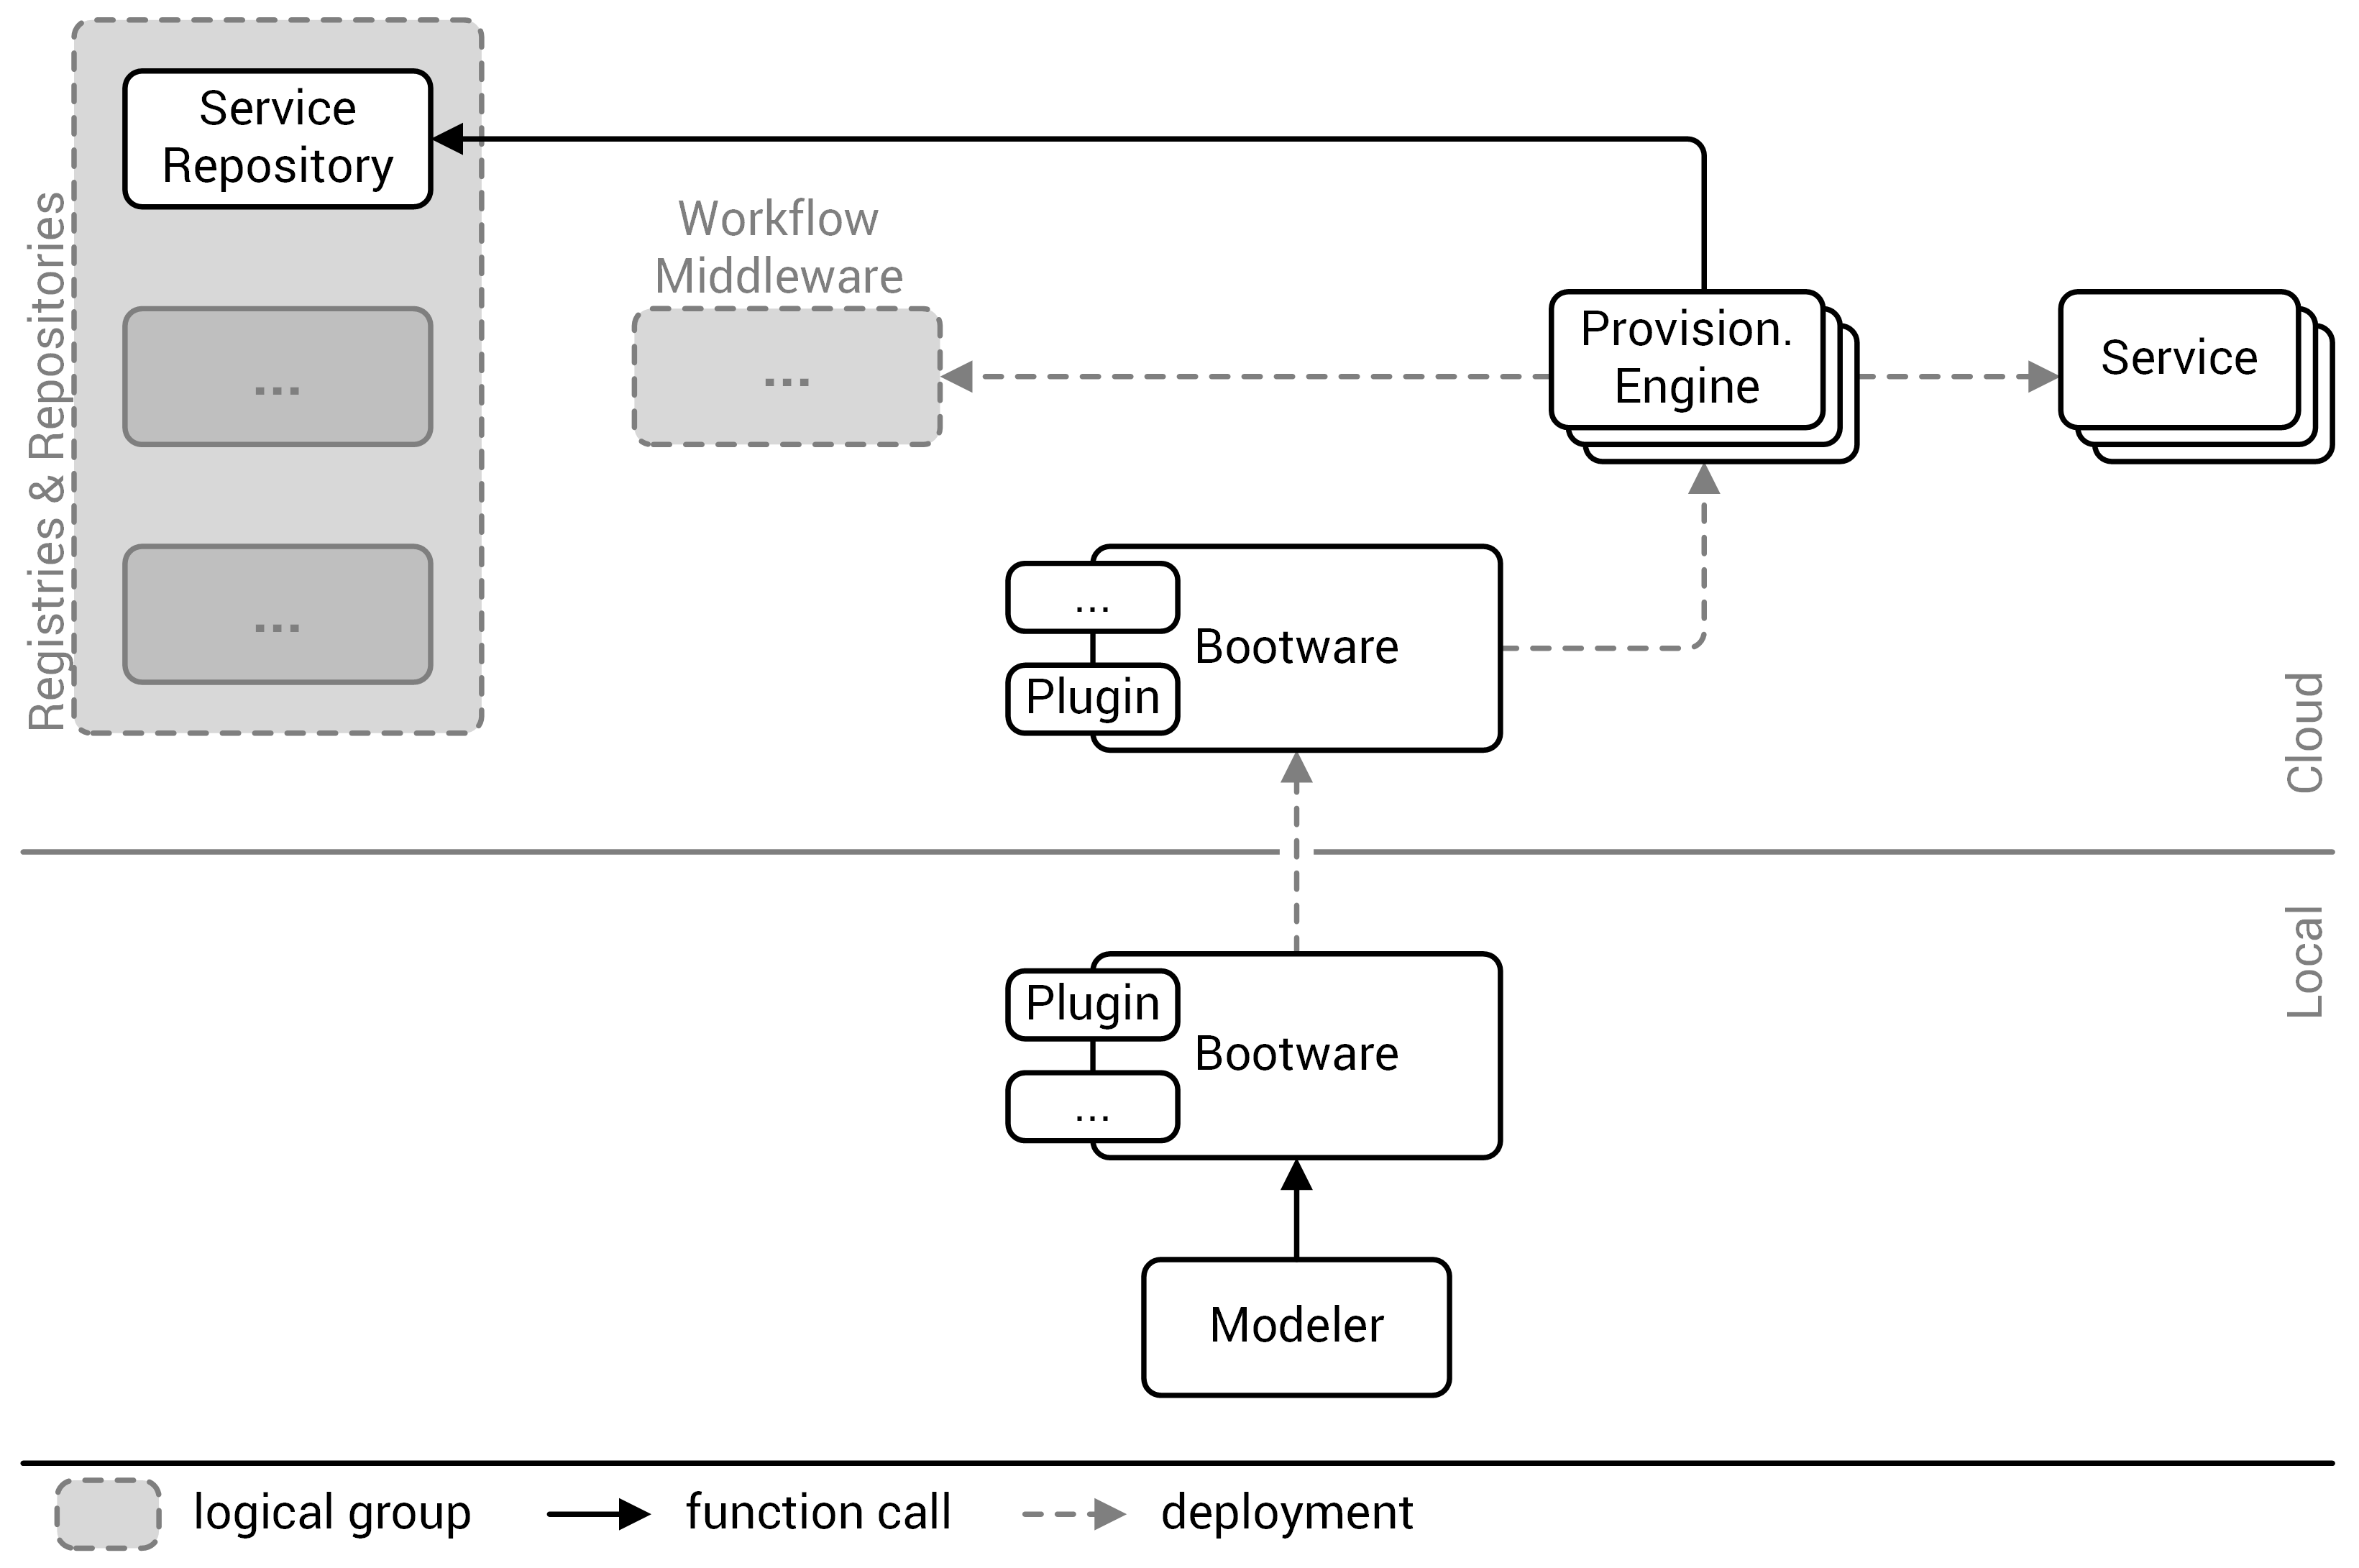
\includegraphics[resolution=600]{design/assets/simple_plugins}
	\caption{Simplified overview of the 2-tier architecture with plugins}
	\label{image:plugins}
\end{figure}

To remedy this situation we introduce a central plugin repository, as shown in \autoref{image:plugin_repository}.
This repository holds all plugins of both components so it eliminates duplicate plugins.
If plugins are added or modified it has only to be done in one place.
Plugin synchronization can happen automatically when the bootware components start, so that the user is no longer involved in plugin management.
The repository also enables easy plugin sharing, which was cumbersome earlier.

\begin{figure}[!htbp]
	\centering
	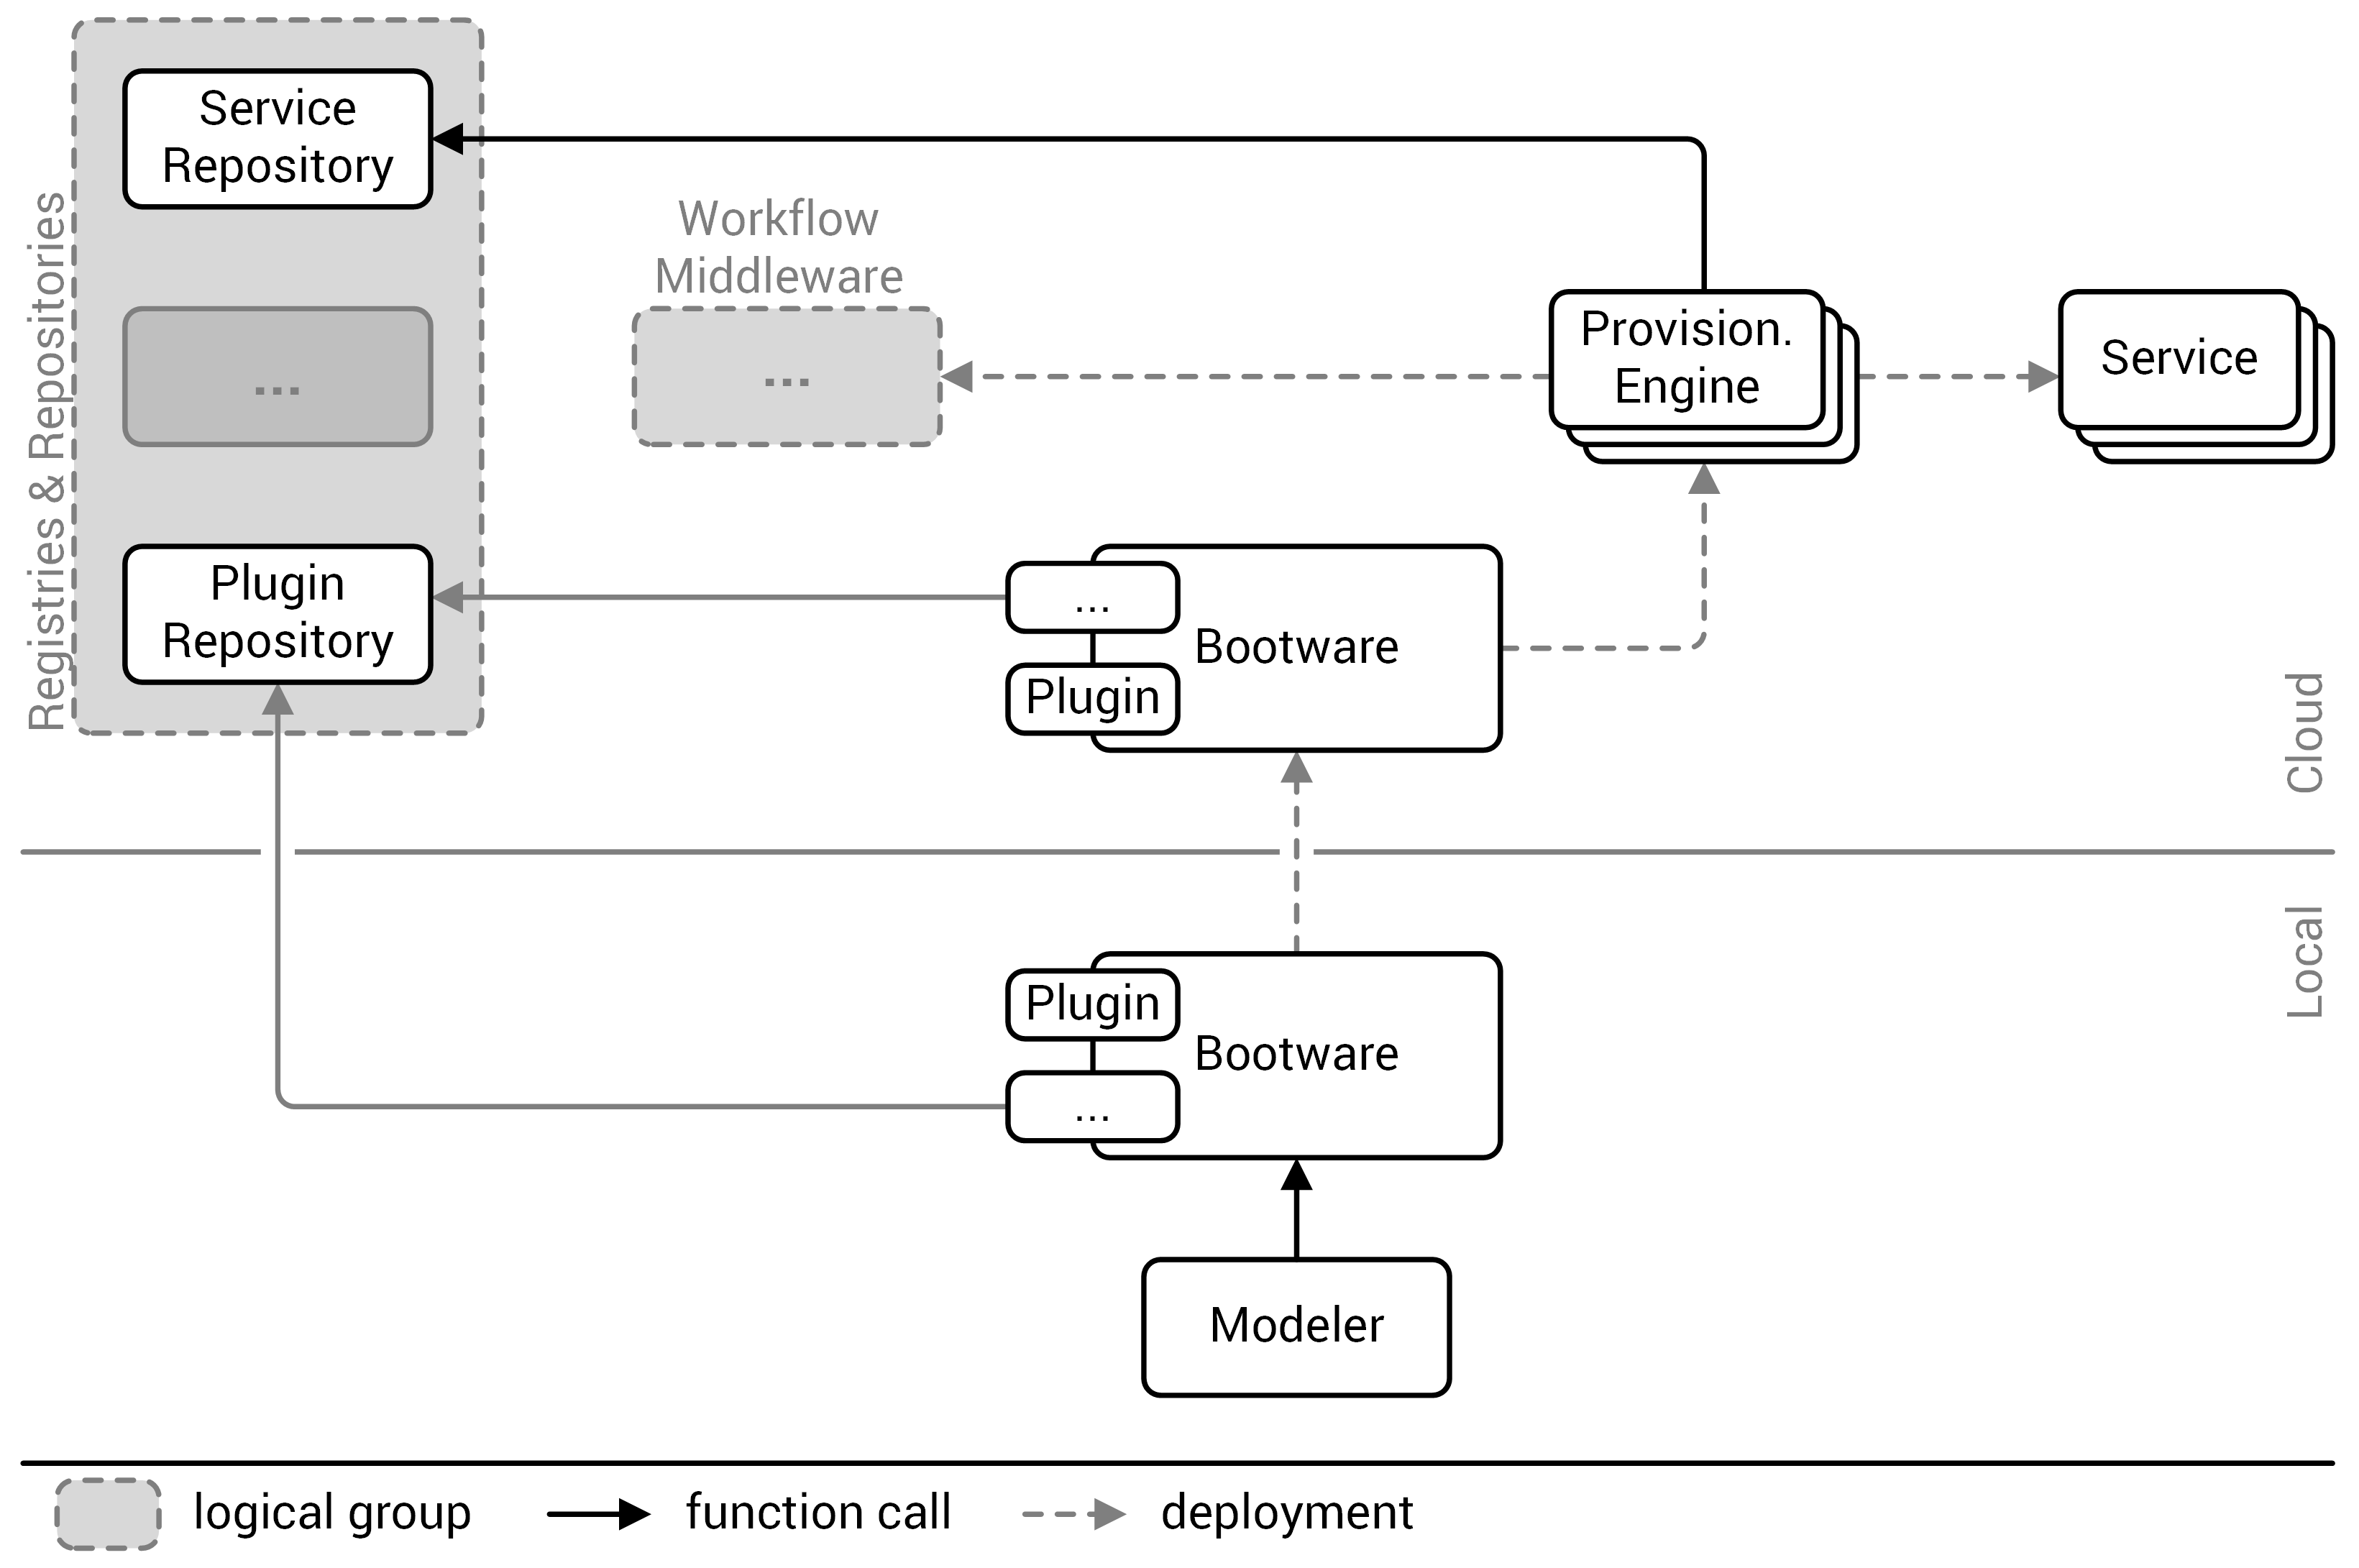
\includegraphics[resolution=600]{design/assets/simple_plugin_repository}
	\caption{Simplified overview of the 2-tier architecture with a plugin repository}
	\label{image:plugin_repository}
\end{figure}

While a central plugin repository is a sensible addition to the proposed bootware architecture, its design and implementation are out of scope of this thesis.
